\chapter[Metas]{Metas}

%O projeto conta com quatro grandes metas principais, passando de criação e desenvolvimento até a parte de lançamento e estabilidade do aplicativo. 

%Como meta inicial, após a elaboração do plano de desenvolvimento do software, faremos a criação e desenvolvimento do aplicativo, parte principal do projeto, buscando robustez já na primeira versão.
% Está vago

%Como segundo passo, trazendo a tarefa que por muitos é dada como mais importante, fazer o teste do aplicativo que vai analisar os mínimos detalhes e possíveis falhas, possibilitando entregar uma versão o mais estável possível. 

%Fazer a divulgação por meio de feiras de ensino, escolas, nas diversas redes sociais e nos sites de ensino, buscando levar o aplicativo não só para as pessoas que querem aprender, mas sim, as que querem ensinar.

%Por último, a tarefa de manter o aplicativo no ar, trabalhando e assegurando que o aplicativo ficará 24 horas disponível e funcional.

% Separar em tópicos
% Aprofundar mais
% Alguns termos estão razos

\section[Cronograma]{Cronograma}

% Como estamos falando de um aplicativo de médio porte, padronizando horário com aplicativos criados ele demoraria de 500 a 800 horas para ser desenvolvido. 

%---- Aqui vai uma tabela ----


O projeto levará 7 meses (1120 horas)

%---- Aqui vai uma tabela ----



\begin{figure}[htb]
	%\caption{\label{gantt}Placa Wiring S}
	\begin{center}
	    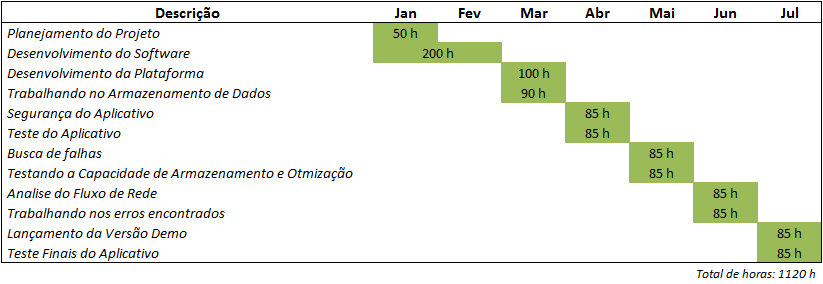
\includegraphics[scale=0.8]{figuras/diagramaGanttCrono}
	\end{center}
	%\legend{Fonte: Site da 3GPP}
\end{figure}

% Não está legal. Montar um cronograma \textit{like a} iniciação científica associando o tópico de metas


% Notas de Aula (CICLO DE VIDA)

% Prazos e Tarefas (Inicio, Desenvolvimento e Final) . Fase 1 discussão, planejamento, desenvolvimento planejamento.

% Cada etapa é uma tarefa. Cada tarefa tem um prazo. (HORAS)

%% CICLO
% Levantamento -> Análise - > Projeto -> Implementação -> Manutenção

% Requisito é etapa "Cada momento é um tempo, cada tempo é uma ação" (PROFESSORA)